\documentclass{article}
\newcommand{\BEAS}{\begin{eqnarray*}}
\newcommand{\EEAS}{\end{eqnarray*}}
\newcommand{\BEQ}{\begin{equation}}
\newcommand{\EEQ}{\end{equation}}
\newcommand{\BIT}{\begin{itemize}}
\newcommand{\EIT}{\end{itemize}}

\newcommand{\eg}{{\it e.g.\ }}
\newcommand{\ie}{{\it i.e.\ }}

\newcommand{\ones}{\mathbf 1}
\newcommand{\zeros}{\mathbf 0}
\newcommand{\reals}{{\mbox{\bf R}}}
\newcommand{\integers}{{\mbox{\bf Z}}}
\newcommand{\symm}{{\mbox{\bf S}}}  % symmetric matrices

\newcommand{\nullspace}{{\mathcal N}}
\newcommand{\range}{{\mathcal R}}
\newcommand{\Rank}{\mathop{\bf Rank}}
\newcommand{\Tr}{\mathop{\bf Tr}}

\newcommand{\sign}[1]{\mathop{\textrm{sgn}}(#1)}
\newcommand{\lambdamax}{{\lambda_{\rm max}}}
\newcommand{\lambdamin}{\lambda_{\rm min}}

\newcommand{\EE}{\mathop{\textrm{E}}}
\newcommand{\Cov}{\mathop{\textrm{Cov}}}
\newcommand{\Prob}{\mathop{\bf Prob}}
\newcommand{\Co}{{\mathop {\bf Co}}} % convex hull
\newcommand{\dist}{\mathop{\bf dist{}}}
\newcommand{\argmin}{\mathop{\rm argmin}}
\newcommand{\argmax}{\mathop{\rm argmax}}
\newcommand{\epi}{\mathop{\bf epi}} % epigraph
\newcommand{\Vol}{\mathop{\bf vol}}
\newcommand{\dom}{\mathop{\bf dom}} % domain
\newcommand{\intr}{\mathop{\bf int}}


\newcommand{\nrm}[1]{\left\lVert#1\right\rVert}
\newcommand{\nrmo}[1]{\left\lVert#1\right\rVert_1}
\newcommand{\nrmt}[1]{\left\lVert#1\right\rVert_2}
\newcommand{\nrmnn}[1]{\left\lVert#1\right\rVert_{*}}
\newcommand{\nrmf}[1]{\left\lVert#1\right\rVert_F}

\newcommand{\myexp}[1]{\mathop{\rm exp}\left\{#1\right\}}
\newcommand{\mylog}[1]{\mathop{\rm log}\left\{#1\right\}}
\newcommand{\questions}{\begin{frame}Questions?\end{frame}}
\newcommand{\LL}{\textrm{LL}}
\newcommand{\KL}{\textrm{KL}}
\newcommand{\HH}{\textrm{H}}
\newcommand{\GG}{\textrm{G}}

\newcommand{\Bound}{\textrm{B}}
\newcommand{\bb}{\mathbf{b}}
\newcommand{\aaa}{\mathbf{a}}
\newcommand{\BB}{\mathbf{B}}
\newcommand{\AAA}{\mathbf{A}}
\newcommand{\CC}{\mathbf{C}}
\newcommand{\cc}{\mathbf{c}}
\newcommand{\mm}{\mathbf{m}}
\newcommand{\MM}{\mathbf{M}}
\newcommand{\nn}{\mathrm{\bf neighbors}}
\newcommand{\pa}[1]{{\textrm{\bf pa}}\left(#1\right)}
\newcommand{\pre}[2]{\mathop{\textrm{\bf pnp}}_{#1}\left(#2\right)}
\newcommand{\logsum}{\textrm{logsum}}

\newcommand{\tth}{{\textrm{th}}}
\newcommand{\xx}{\mathbf{x}}
\newcommand{\mmu}{\mathbf{\mu}}
\newcommand{\yy}{\mathbf{y}}
\newcommand{\zz}{\mathbf{z}}
\newcommand{\dd}{\mathbf{d}}
\newcommand{\new}{\textrm{new}}
\newcommand{\old}{\textrm{old}}
\newcommand{\fpr}{\textrm{FPR}}
\newcommand{\tpr}{\textrm{TPR}}
\newcommand{\auc}{\textrm{AUC}}
\newcommand{\yyi}{\yy_i}
\newcommand{\xxi}{\xx_i}
\newcommand{\vvec}[2]{\left[ \begin{array}{c} \mathbf{#1}\\ \mathbf{#2} \end{array}\right]}
\newcommand{\mmat}[4]{\left[ \begin{array}{cc} \mathbf{#1}&\mathbf{#2}\\ \mathbf{#3}&\mathbf{#4} \end{array}\right]}
\newcommand{\xyvec}{\left[ \begin{array}{c} \xx\\\yy \end{array} \right]}
\newcommand{\xyvecc}{\left[ \begin{array}{c} x^1\\y^1 \end{array} \right]}
\newcommand{\eye}{   \left[ \begin{array}{cc} 1 & 0 \\ 0 & 1 \end{array}\right]}
\newcommand{\bket}[2]{\left\langle#1,#2\right\rangle}
\newcommand{\bbket}[2]{\left\llangle#1,#2\right\rrangle}
\newcommand{\redq}{\textcolor{red}{q}}
\newcommand{\blup}{\textcolor{blue}{p}}
\newcommand{\BIEA}{\begin{IEEEeqnarray*}}
\newcommand{\EIEA}{\end{IEEEeqnarray*}}
\newcommand{\BIEAN}{\begin{IEEEeqnarray}}
\newcommand{\EIEAN}{\end{IEEEeqnarray}}
\newcommand{\pmin}{\mathop{\textrm{minimize}}}
\newcommand{\psubjto}{\textrm{subject to}}
\newcommand{\WW}{\mathbf{W}}
\newcommand{\ww}{\mathbf{w}}
\newcommand{\YY}{\mathbf{Y}}
\newcommand{\XX}{\mathbf{X}}
\newcommand{\UU}{\mathbf{U}}
\newcommand{\uu}{\mathbf{u}}
\newcommand{\VV}{\mathbf{V}}
\newcommand{\vv}{\mathbf{v}}
\newcommand{\PP}{\mathbf{P}}
\newcommand{\pp}{\mathbf{p}}
\newcommand{\rr}{\mathbf{r}}
\newcommand{\RR}{\mathbf{R}}
\newcommand{\ee}{\mathbf{e}}
\newcommand{\BA}{\mathbf{A}}

\newcommand{\aalpha}{{\boldsymbol\alpha}}
\newcommand{\llambda}{{\boldsymbol\lambda}}
\newcommand{\ddelta}{{\boldsymbol\delta}}
\newcommand{\otherwise}{\textrm{otherwise}}
\newcommand{\answer}{\fbox{\tt answer} }
\newcommand{\abs}[1]{\left| #1 \right|}

\newcounter{problemCtr}
\newcommand{\newproblem}[1]{\hrule\paragraph{Problem \theproblemCtr (#1)}\stepcounter{problemCtr}}


\newcounter{HW}

\usepackage{amsthm}
\usepackage{graphicx}
\usepackage{natbib}
\usepackage{algorithm}
\usepackage{algorithmic}
\usepackage{amsmath}
\usepackage{hyperref}


\newtheorem{remark}{Remark}
\newtheorem{lemma}{Lemma}
\newtheorem{definition}{Definition}
\newtheorem{proposition}{Proposition}
\newtheorem{assumption}{Assumption}
\newtheorem{corollary}{Corollary}
\newtheorem{theorem}{Theorem}


\usepackage{listings}
\setcounter{HW}{1}
\begin{document}
\lstset{language=Python}
\lstset{basicstyle=\ttfamily}
\lstset{tabsize=4}
\lstset{columns=fullflexible}

\author{Markus Padourek}
\title{COMP  790-124, HW\theHW}
\maketitle



\newproblem{0.01pt} Open \texttt{hw\theHW.tex}, replace ``Wile E. Coyote'' with your name. Run
\texttt{pdflatex hw\theHW.tex}, look at hw\theHW.pdf, and confirm that your name is in the right place.


\newproblem{1pt}
\begin{enumerate}
\item Plot the sigmoid function in MATLAB using script
\begin{verbatim}
z = np.arange(-5, 5, 0.1)
fz = 1. / (1 + np.exp(-z))
plt.plot(z, fz, linewidth=3)
plt.xlabel('z')
plt.ylabel('f(z)')  # we always label axes, yes we do!
hwplotprep()
plt.savefig('sigmoid.pdf')
\end{verbatim}
Find the resulting figure in file {\tt sigmoid.pdf}.
b) In hw\theHW.tex, find the segment of the file that sets up the first figure -- it starts with {\tt \textbackslash begin\{figure\}} and ends with  {\tt \textbackslash end\{figure\}}.
\item Inside this segment  replace {\tt emptiness.pdf} with {\tt sigmoid.pdf}.
\item Change the text under {\tt \textbackslash caption} -- right now it says ``This is emptiness, it earns no points.'' -- to say what the figure is about.
\item Remake hw\theHW.pdf by running in shell/command prompt
z
     \texttt{pdflatex hw\theHW.tex}

and check that your plot and caption are now in.
\end{enumerate}


\begin{figure}[H]
\begin{center}
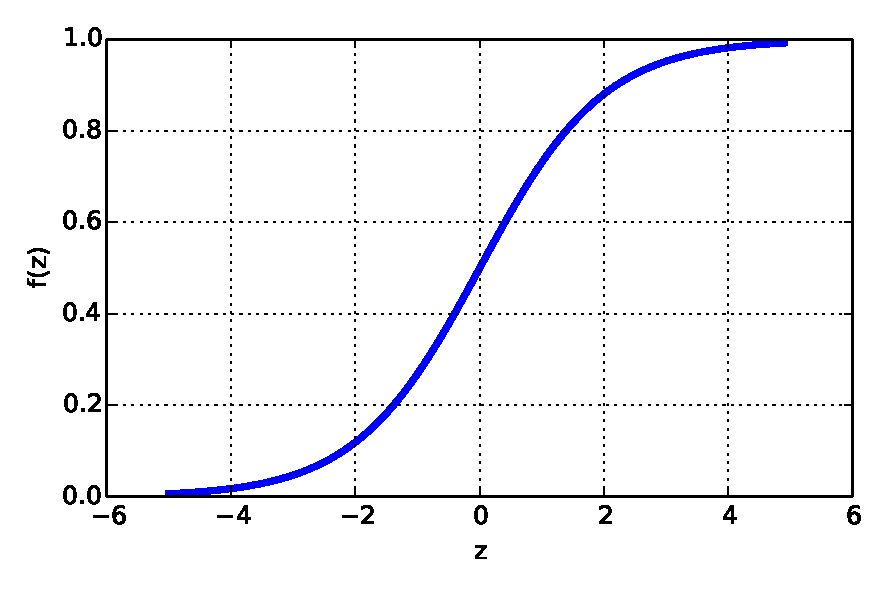
\includegraphics[scale=0.5]{sigmoid.pdf}
\caption{The Sigmoid function.}
\end{center}
\end{figure}

\hrule

\newproblem{1pt}
Fill in the first derivative and second derivative of sigmoid function in the hw\theHW.tex.

The first derivative
\[
\frac{d f(z)}{dz} =  \frac{e^{-z}}{(1 + e^{-z})^2}.%here goes your derivative, but before the % character otherwise it will be commented out
\]

\[
\frac{d^2 f(z)}{dz^2} = \frac{2 * e^{-2z}}{(1 + e^{-z})^3} - \frac{e^{-z}}{(1 + e^{-z})^2}
\]

You might have to consult an intro to \LaTeX in order to figure out how to format your math.

\newproblem{1pt}
Write a MATLAB function that implements computation  of the first derivative of $f$ at a particular point. You just did the math for this.
Here is a function that is {\em right}
\begin{lstlisting}
import numpy as np
def dsigmoid(z):
    d = np.exp(-z) / (1 + np.exp(-z)) ** 2
    return d
\end{lstlisting}
Correct hw\theHW.tex by replacing {\tt ...} above with the correct MATLAB code to compute expression you obtained in previous problem.

Crate a file {\tt dsigmoid.py} that {\em correctly} computes the first derivative.

\newproblem{1pt}

We will use your function {\tt dsigmoid.py} to plot the first derivative.
\begin{lstlisting}
zs = np.arange(-5, 5, 0.01)
ds = np.arange(zs.shape[0], dtype=np.float64)
for i in range(zs.shape[0]):
    ds[i] = dsigmoid(zs[i])


plt.plot(zs, ds, linewidth=3)
plt.xlabel('z')
plt.ylabel('df(z)')
hwplotprep()
plt.savefig('dsigmoid.pdf')
\end{lstlisting}

Find the resulting plot in file {\tt dsigmoid.pdf}. In hw\theHW.tex replace {\tt emptiness.pdf} with {\tt dsigmoid.pdf} . Change the
caption in the figure to say what the figure is about. Remake hw\theHW.pdf and check that your plot has made it in.
\begin{figure}[H]
\begin{center}
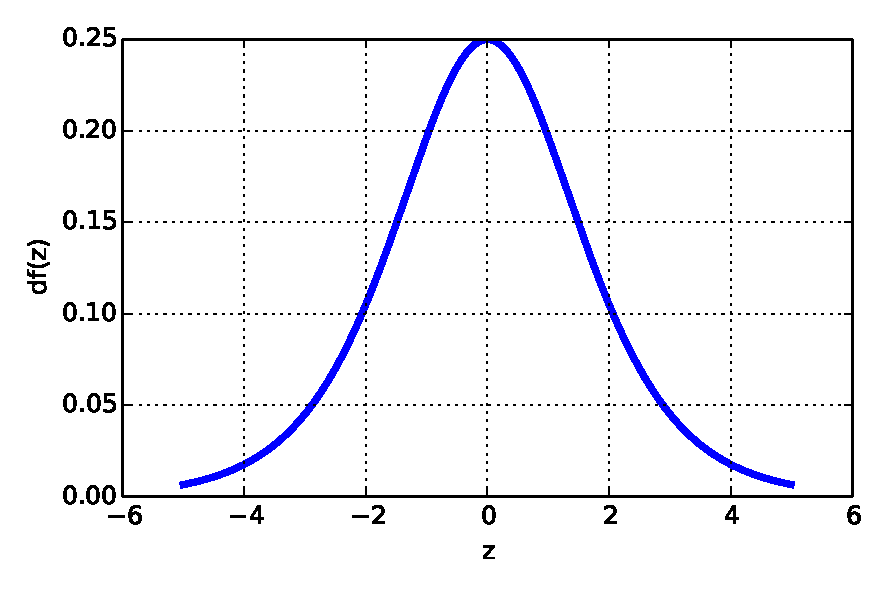
\includegraphics[scale=0.5]{dsigmoid.pdf}
\caption{This is the first derivative of the Sigmoid function.}
\end{center}
\end{figure}


\newproblem{1pt}
We can approximate derivatives numerically
\[
\frac{df(z)}{dz}\approx \frac{f(z+h) - f(z)}{h}
\]
where the right-side of this approximate equality is called {\em finite difference} approximation. Unlike derivative definition we do not need $h$ to be infinitesimal, just a small value. The numerical approximation of a derivative is tremendously useful trick to check you derivative, gradients, Jacobians, Hessians etc. Make sure that you understand what it does.

We will use this approximation to check your derivatives. Here is a function that computes approximately the derivatives of sigmoid
\begin{lstlisting}
def fdsigmoid(z):
    f0 = 1 / (1 + np.exp(-z))
    f1 = 1 / (1 + np.exp(-(z + 1e-5)))
    d = (f1 - f0) / 1e-5
    return d
\end{lstlisting}
Save this function into a file names \texttt{fdsigmoid.py}.

Try the following code
\begin{lstlisting}
zs = np.random.randn(100)
err = np.empty(zs.shape[0])
for i in range(zs.shape[0]):
    err[i] = dsigmoid(zs[i]) - fdsigmoid(zs[i])
plt.figure()
plt.hist(err, 30)
hwplotprep()
plt.savefig('hist.pdf')
\end{lstlisting}
The code above samples 100 normally distributed values and computes the finite differences approximation and the derivative you derived and implemented and then plots histogram of errors.

Find the resulting plot in file {\tt hist.pdf}. In hw\theHW.tex replace {\tt emptiness.pdf} with {\tt hist.pdf} . Change the
caption in the figure to say what the figure is about. Remake hw\theHW.pdf and check that your plot has made it in.
\begin{figure}[H]
\begin{center}
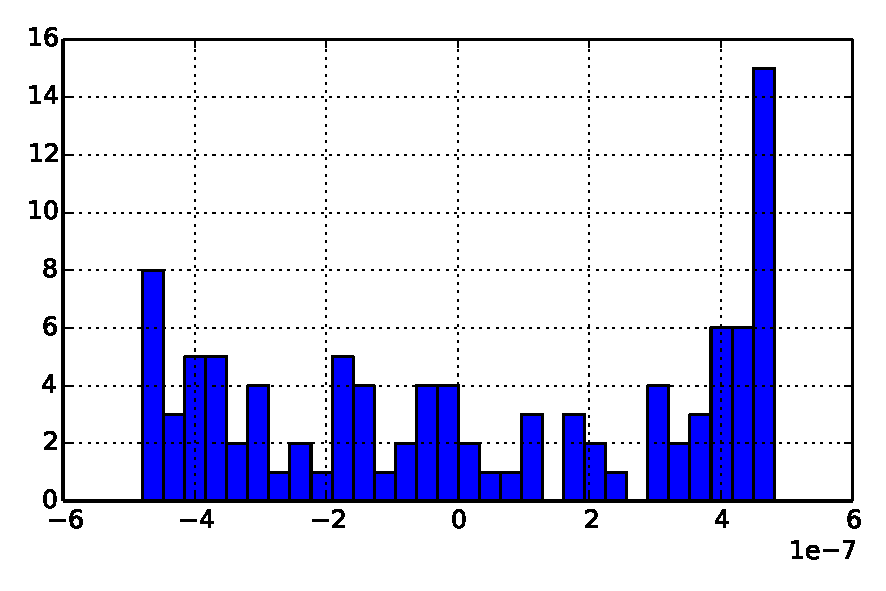
\includegraphics[scale=0.5]{hist.pdf}
\caption{Groups the error into 30 equal intervals and displays their frequency}
\end{center}
\end{figure}



\begin{remark} The errors ranges, roughly, between \( -5*10^{-7}\) and \(5*10^{-7}\) .
\end{remark}

\newproblem{1pt}
From Taylor's theorem (first year calculus) we can obtain
\[
f(z+h) = f(z) + \frac{df(z)}{dz}h + \frac{1}{2}\frac{d^2f(z)}{d^2z}h^2 + O(h^3).
\]
Derive a bound on the error of the finite differences approximation using the above expression. You can use big O notation to express this bound.
\[
\textrm{Err}(z_0,h) = \abs{\frac{f(z_0+h) - f(z_0)}{h} - \frac{df(z_0)}{dz}} \leq O(h)
\]

Specifically for sigmoid function plug in appropriate derivative on the right hand side of the inequality. If $h=10^{-5}$ and $z_0 = 0$ the error of the finite difference should be about \(9.464*10^{-12}\) .
Does this agree with the histogram of error that is in the figure above? Yes.

\newproblem{1pt}
Let
\BEQ\label{eq:pz}
f(z) = \frac{1}{1 + \myexp{-z}} = p
\EEQ
express $z$ in terms of $p$
\[
z = -\mylog{\frac{1-p}{p} }.
\]
Now suppose
\BEQ\label{eq:qz}
\frac{\myexp{-z}}{1 + \myexp{-z}} = q
\EEQ
and express $z$ in terms of $q$
\[
z = \mylog{\frac{1-q}{q} }.
\]
Given Eqs.\eqref{eq:pz},\eqref{eq:qz} express $q$ in terms of $p$
\[
q = 1-p.
\]
Express $f(-z)$ in terms of $f(z)$
\[
f(-z) = \frac{1}{1 + \myexp{z}}.
\]
Hint: the manipulations that are useful here are either subtraction from 1 (as in $1-x$), computing inverse (as in $\frac{1}{x}$), and taking logarithm (as in $\log(x)$).

\section*{Log of sigmoid}
\newproblem{1pt}
Let $g(z)$ be log of sigmoid function
\[
g(z) = \mylog{ \frac{1}{1+ \myexp{-z}} }.
\]
Compute its derivative and fill it in here
\[
\frac{dg(z)}{dz} =   \frac{\myexp{-z}}{1 + \myexp{-z}}.%here goes your derivative of log sigmoid, but before the % character otherwise it will be commented out
\]
Check your derivative by comparing its value to the finite difference approximation.


\newproblem{1pt}
Compute second derivative of $g(z)$
\[
\frac{dg(z)}{dz} =  - \frac{\myexp{-z}}{(1 + \myexp{-z})^2}.%here goes your derivative of log sigmoid, but before the % character otherwise it will be commented out
\]
Check the second derivative by comparing its value to the finite difference of the {\em first} derivatives you computed above.


\newproblem{1pt}
Let the dataset be specified by $\mathcal{D} = \left\{ (\xx_i,y_i):i=1,\dots,n \right\}$. We specify conditional probability of $y$
\BEQ \label{eq:plr}
p(y | \xx_i,\beta_0,\beta) = \frac{1}{1 + \myexp{-y_i(\beta_0 + \bket{\beta}{\xx_i})}}
\EEQ
Write a matlab function that computes log probability of label $y$ given a vector of features $\xx$ and $\beta_0,\beta$.
\begin{lstlisting}
import numpy as np
def logProbLogReg(self, y, X, beta0, beta):
	logP = np.log(1 / (1 + np.exp(-y * (beta0 + np.dot(X, beta))))
	return logP[0, 0]
\end{lstlisting}
Now write a matlab function that uses the above function to compute log probability of label $+1$ for a vector of features $\xx$ and $\beta_0,\beta$
\begin{lstlisting}
def predictY(X, beta0, beta):
	logProbY = logProbLogReg(1,X,beta0,beta);
	if logProbY > np.log(0.5):
		predY = 1
	else:
		predY = -1
	return predY
\end{lstlisting}


\newproblem{1pt}
Given Eq.\eqref{eq:plr} we can write out log-likelihood
\BEQ \label{eq:ll}
\textrm{LL}(\beta_0,\beta;\mathcal{D}) = \sum_i \log \frac{1}{1 + \myexp{-y_i(\beta_0 + \bket{\beta}{\xx_i})}}.
\EEQ
Now using function $\texttt{logProbLogReg}$ that you obtained for the previous problem, write a matlab function that computes loglikelihood
\begin{lstlisting}
def LogLikLogReg(y, X, beta0, beta):
	val = 0
	for i in range(y.shape[1]):
		val += logProbLogReg(y[i], X[i, :], beta0, beta)
	return val
\end{lstlisting}
\newproblem{1pt}
Write a function that computes gradient of log-likelihood of logistic regression Eq.\eqref{eq:ll}
\begin{lstlisting}
def dLogLikLogReg(self, y, X, beta0, beta):
	dbeta = np.empty(beta.shape)
	dbeta0 = sum((1 - 1 / (1 + np.exp(-y * (beta0 + np.dot(X, beta))))) * y)[0]
	for p in range(beta.shape[0]):
		e = (1 - 1 / (1 + np.exp(-y * (beta0 + np.dot(X, beta))))) 
		dbeta[p, 0] = sum(e * y * X[:, p][:, np.newaxis])
	return dbeta0, dbeta
\end{lstlisting}
You can make sure that your implementation is correct using the finite differences trick.
\newproblem{1pt}
Implement a gradient ascent algorithm for fitting logistic regression and paste it below.
\begin{lstlisting}
from logProbability import logProbability
import numpy as np
from scipy.io import loadmat

def fitLogReg(y, X):
	beta0 = 0
	beta = np.random.randn(X.shape[1], 1)
	s = 1e-5
	i = 0
	MAXITER = 200
	#functon dLogLikLogReg() is in a class, so creating an instance of that
	lP = logProbability()
	while i < MAXITER:
		beta0New, betaNew = lP.dLogLikLogReg(y, X, beta0, beta)
		beta0 += s * beta0New
		beta += s * betaNew
		i += 1
	return beta0, beta
\end{lstlisting}
Run it with fixed step size $s=10^{-5}$, for 2000 iterations, on data stored in \texttt{hw\theHW.mat}.
Note that \texttt{load hw\theHW.mat} loads the $y$ and $X$ variables, on which you can run by issuing command
\texttt{[beta0,beta] = fitLogReg(y,X)}.
Report resulting $\beta_0,\beta$
\begin{lstlisting}
beta0 = 0.0165875601408
beta = [ -7.94603664e-01   6.44421758e-01  -9.61391742e-01   1.06937019e+00
   1.25019519e+00  -9.28803658e-02  -1.08953222e+00  -5.76315912e-01
   1.03434783e+00   8.35273564e-02   6.53991220e-01  -8.85354863e-02
   1.38944196e-01  -6.82042722e-02   1.52336181e+00  -1.94079096e+00
  -9.47058446e-01  -6.06370794e-01  -1.92000125e+00   1.96388643e-01
  -1.63501668e+00  -1.10440445e+00  -1.74322582e+00   5.76609515e-01
   2.72144090e+00   4.36680029e-01   1.11006795e+00   2.87044833e-01
   5.17655091e-01   9.72082232e-01   2.22033898e+00  -8.60831281e-01
  -1.44883333e+00   1.32604611e+00   1.30908073e+00  -4.19314637e-01
  -1.25747017e+00  -1.99007411e+00  -1.33023671e+00  -6.26517811e-02
  -1.14131764e+00  -1.07772700e+00   1.33177224e+00  -2.04504144e-01
  -1.26311558e+00  -1.00069979e+00  -1.57158209e+00  -7.72912071e-01
  -1.07518793e+00  -1.66871900e+00   6.35135519e-01   1.11737791e-01
   9.51466378e-01  -1.38972471e+00   7.25131840e-01   1.01024849e+00
   4.95679854e-01  -1.03828798e+00  -2.86016598e+00   2.82723322e-02
   5.84770128e-01  -1.65019508e-01   1.11914941e+00   3.45791033e-01
   2.47709907e-02   1.48863723e+00  -1.26812599e+00   9.71599692e-01
   3.24199832e-01   9.23761813e-01   1.44076772e+00   1.15028143e+00
   5.73586263e-01   1.39245075e+00  -1.38585823e+00   5.44671024e-01
   8.92444161e-04   1.69826753e+00  -1.94120611e+00  -1.54894876e+00
   3.55364013e-01  -1.83551658e+00  -1.18020903e+00   6.53574856e-01
   1.95278213e-01  -1.27846452e+00   1.49864456e+00  -5.16285341e-01
  -3.88012600e-01  -2.08024944e+00  -7.84315905e-01  -4.42029501e-02
  -5.18336496e-01  -1.30306486e+00   6.74282589e-01  -1.49525668e+00
   5.35003612e-01   9.47754465e-01   1.19589829e+00   1.59268045e+00
  -4.18847821e-01  -5.98149032e-01   6.54757066e-01   8.05947430e-01
   6.48798157e-01  -1.26261903e+00  -8.18593936e-01   1.42383704e+00
  -1.52270921e+00  -1.20783789e+00   7.01470048e-01   4.86422803e-02
  -3.67682495e-01  -1.34721986e+00  -4.18474059e-01  -3.93564357e-01
  -4.11907916e-01  -7.64144055e-01   1.58961903e-01   3.59366105e-02
  -1.49257319e+00   3.03401205e-01  -5.04996804e-01   1.70453702e+00
  -1.02545625e-01  -2.24776072e+00  -6.74566908e-01   4.67050757e-01
   6.19506995e-01  -1.26484970e+00  -6.01368623e-01   1.17447384e+00
  -3.42122060e-01   1.32773284e-01  -6.44389597e-01   5.61390936e-01
  -2.95755704e-01  -1.11365436e+00  -8.36988761e-01   1.24821616e+00
   3.96597113e-02   1.74831624e+00   1.07572472e+00  -9.28336249e-01
  -8.81577649e-01  -1.80186704e+00  -1.27443015e-01   1.49524653e+00
   2.57661148e-01  -1.93897387e-01  -6.21616446e-01   1.15156073e+00
   1.54834219e+00   7.10554318e-01   1.50314041e+00   6.62455788e-01
  -1.12235745e+00  -2.97158213e-01   1.17762898e-01   6.69539321e-01
  -5.32395944e-01  -6.07290389e-01  -4.35157875e-01   5.47405044e-01
  -4.10750127e-01   1.44827057e-01  -1.80625362e-01   1.71956098e+00
  -4.82979252e-02   7.40805422e-01  -5.82085177e-01  -8.21214676e-01
  -1.51100009e-01  -1.32751950e+00   6.98488601e-01  -1.56884655e+00
   1.41248643e+00  -9.82093362e-01   1.02666023e+00  -5.04932165e-01
   1.00355557e+00   1.35110919e-01   1.53359319e+00   1.66435846e+00
  -1.46036071e+00  -3.06669503e-01  -6.11713757e-01  -1.09198911e+00
   2.71287017e-01   2.10125148e+00   8.36003621e-01  -9.36137761e-01
  -1.15286486e-01   4.36996686e-01  -6.06568449e-02   9.61424208e-01
  -9.74298866e-01   4.42222541e-01  -3.26335047e-01   1.14773194e+00
  -1.58574188e-01  -8.19436922e-01   8.03338979e-01   5.35920312e-01
  -3.86382727e-01   6.05720296e-02  -9.13374591e-01  -1.16775091e+00
  -9.10929246e-01  -1.14991979e+00   3.07149965e-01   1.30932494e-01
  -4.39035582e-01   8.96196950e-01  -6.70354588e-01   1.25062331e+00
   7.80640753e-02  -9.86954441e-01  -1.17791783e+00   6.97320936e-01
   1.54730482e+00   8.32054559e-01   1.48391200e+00   7.35299520e-01
  -7.32273567e-01  -4.28218364e-01  -1.52779856e+00  -3.76419210e-01
  -1.22247706e-01  -3.30737671e-01  -8.11488151e-01   1.41684623e+00
  -2.74436858e-01  -3.82126206e-01  -4.93483177e-02   5.60979378e-01]
\end{lstlisting}
\newproblem{1pt}
Implement estimation of prediction error using cross validation
\begin{lstlisting}
from scipy.io import loadmat
import numpy as np
from sklearn.cross_validation import KFold
from gradientAscent import GradientAscentLogReg
from logProbability import *


mat = loadmat('hw1.mat')
X = np.array(mat['X']).T
y = np.array(mat['y']).T
K = 5
N = y.shape[0]
err = np.zeros(K)
k = 0
ga = GradientAscentLogReg()
lp = logProbability()

np.random.seed(1)
kf = KFold(N, n_folds=K)
for trainIndex, testIndex in kf:
	XTrain, XTest = X[trainIndex], X[testIndex]
	yTrain, yTest = y[trainIndex], y[testIndex]

	beta0, beta = ga.fitLogReg(yTrain, XTrain)

	for i in range(yTest.shape[0]):
		yPred = lp.predictY(XTest, beta0, beta)
		err[k] += (np.abs(yPred - yTest[i]) / 2)
	k += 1
cvErr = np.sum(err) / y.shape[0]
print(cvErr)
\end{lstlisting}
Once done, run this on data stored in \texttt{hw\theHW.mat}. The cross-validation estimate of error on that dataset is 0.2643.
\end{document}
